%% 본문(document) 안에서 글쓰다가 엔터 두번(줄바꿈 명령어) 치고 다시 글쓰면, paragraph 바뀌는 거임. 
%% 그럼 새 paragraph은 pdf 상에서 이전 paragraph 바로 아랫줄로 위치하게 되고 자동으로 indentation 적용됨.
%% 두 줄 띄우고 싶으면 \\(빈 줄 입력 명령어) 입력하고 엔터 두 번(줄바꿈 명령어) 쓰면 됨.
%% \[ \] 사용하면, 두 번 엔터 안 쓰고 그냥 한 번 엔터 눌르고 본문 이어가도 줄바꿈 자동 적용됨.

%%%%%%%%%%%%%%%%%%%%%%%%%%%%%%%%%%%%%%%%%%%%%%%% Preamble %%%%%%%%%%%%%%%%%%%%%%%%%%%%%%%%%%%%%%%%%%%%%%%%
% 메타 정보 입력 섹션
\documentclass{article} % 문서 타입 정의

\usepackage{amsmath, amssymb, geometry} % 사용할 패키지 import
\usepackage{graphicx}  % 이미지 삽입을 위한 패키지
\usepackage{caption}   % 캡션 조절용 (선택)
\usepackage{booktabs}  % 표에서 \toprule, \midrule, \bottomrule 사용을 위한 패키지

\geometry{
    a4paper,
    left=25.4mm,
    right=25.4mm,
    top=25.4mm,
    bottom=25.4mm,
    } % 문서 크기 및 여백 설정
\linespread{1.3} % 줄 간 간격 조절 ; default : 1.0

\title{\vspace{0cm} Assignment \#1: Review of Numerical Methods \\ and Basics of Optimization} % 제목
% \author{Course \hfill: Numerical Optimization \\ Name : Chiyoung Kwon % 내 신상
%  \\ ID : 261258263 \\ Department : Mechanical Engineering \\ Program : PhD}
\date{} % 작성일자 ; 비워져있으면 출력 안됨

%%%%%%%%%%%%%%%%%%%%%%%%%%%%%%%%%%%%%%%%%%%%%%%% Document %%%%%%%%%%%%%%%%%%%%%%%%%%%%%%%%%%%%%%%%%%%%%%%%
% 본문 섹션
\begin{document} % 문서 본문 시작
\maketitle{ % 위에서 쓴 제목, 내 신상, 작성일자 실제로 출력시키는 명령어
    \begin{flushright} % 오른쪽 정렬
        {
        \vspace{-1.5cm}
        Sep 24th, 2025 \\
        \vspace{2mm}
        Course : Numerical Optimization \\ Name : Chiyoung Kwon \\ ID : 261258263 \\
        Department : Mechanical Engineering \\ Program : PhD
        }
    \end{flushright}
    }
{
    \noindent 1. Consider the following function and do the following (by hand):
    \[ f(\mathbf{x}) = 2x_1^2 - 3x_2^2 + 4x_1x_2 + (x_3 + 2)^2 + 4x_1 \] 
    \noindent (a) What are the gradient and Hessian of $ f(\mathbf{x}) $?
    \[ \nabla^T f(\mathbf{x}) = \begin{bmatrix} \frac{\partial f}{\partial x_1} \\
        \frac{\partial f}{\partial x_2} \\ \frac{\partial f}{\partial x_3} \end{bmatrix} 
        = \begin{bmatrix} 4x_1 + 4x_2 + 4 \\ -6x_2 + 4x_1 \\ 2x_3 + 4 \end{bmatrix} \]
    \[ \mathbf{H}(\mathbf{x}) = \nabla(\nabla^T f(\mathbf{x})) = \begin{bmatrix}
        \frac{\partial^2 f(\mathbf{x})}{\partial x_1^2} & \frac{\partial^2 f(\mathbf{x})}{\partial x_1 \partial x_2} & \frac{\partial^2 f(\mathbf{x})}{\partial x_1 \partial x_3} \\
        \frac{\partial^2 f(\mathbf{x})}{\partial x_2 \partial x_1} & \frac{\partial^2 f(\mathbf{x})}{\partial x_2^2} & \frac{\partial^2 f(\mathbf{x})}{\partial x_2 \partial x_3} \\
        \frac{\partial^2 f(\mathbf{x})}{\partial x_3 \partial x_1} & \frac{\partial^2 f(\mathbf{x})}{\partial x_3 \partial x_2} & \frac{\partial^2 f(\mathbf{x})}{\partial x_3^2}
    \end{bmatrix}
    = \begin{bmatrix}
        4 & 4 & 0 \\
        4 & -6 & 0 \\
        0 & 0 & 2
    \end{bmatrix} \]

    \noindent (b) What are the stationary point(s) of $ f(x) $? \\

    The gradient of function at the stationary point is zero. Let stationary point $\mathbf{x^*}$
    \[ \rightarrow \nabla f(\mathbf{x^*}) = \mathbf{0} \]

    \[ \rightarrow \begin{bmatrix} 4x^*_1 + 4x^*_2 + 4 \\ -6x^*_2 + 4x^*_1 \\ 2x^*_3 + 4 \end{bmatrix} = \begin{bmatrix} 0 \\ 0 \\ 0 \end{bmatrix} \]
    
    \[ \rightarrow \begin{bmatrix}
        4 & 4 & 4 \\
        4 & -6 & 0 \\
        0 & 0 & 2
    \end{bmatrix} \begin{bmatrix}
        x^*_1 \\ x^*_2 \\ x^*_3
    \end{bmatrix} = \begin{bmatrix}
        0 \\ 0 \\ -4
    \end{bmatrix} \]

    By Gaussian elimination process,

    \[ \rightarrow \begin{bmatrix}
        4 & 4 & 4 \\
        4 & -6 & 0 \\
        0 & 0 & 1
    \end{bmatrix} \begin{bmatrix}
        x^*_1 \\ x^*_2 \\ x^*_3
    \end{bmatrix} = \begin{bmatrix}
        8 \\ 0 \\ -2
    \end{bmatrix} \]

    \[ \rightarrow \begin{bmatrix}
        1 & 1 & 0 \\
        0 & -10 & 0 \\
        0 & 0 & 1
    \end{bmatrix} \begin{bmatrix}
        x^*_1 \\ x^*_2 \\ x^*_3
    \end{bmatrix} = \begin{bmatrix}
        2 \\ -8 \\ -2
    \end{bmatrix} \]

    \[ \rightarrow \begin{bmatrix}
        1 & 0 & 0 \\
        0 & 1 & 0 \\
        0 & 0 & 1
    \end{bmatrix} \begin{bmatrix}
        x^*_1 \\ x^*_2 \\ x^*_3
    \end{bmatrix} = \begin{bmatrix}
        1.2 \\ 0.8 \\ -2
    \end{bmatrix} \]

    \[ \therefore \mathbf{x^*} = \begin{bmatrix}
        1.2 \\ 0.8 \\ -2
    \end{bmatrix} \]

    \noindent (c) Is the Hessian positive-definite? \\

    To determine if Hessian is positive-definite, the eigenvalues of Hessian should be evaluated.
    Let $\mathbf{x^*}$ eigenvector and $\lambda$ eigenvalues.

    \[ \rightarrow (\mathbf{H} - \lambda \mathbf{I}) \mathbf{x^*} = \mathbf{0} \]

    \[ \rightarrow \begin{bmatrix}
        4 - \lambda & 4 & 0 \\
        4 & -6 - \lambda & 0 \\
        0 & 0 & 2 - \lambda
    \end{bmatrix} \begin{bmatrix}
        x^*_1 \\ x^*_2 \\ x^*_3
    \end{bmatrix} = \begin{bmatrix}
        0 \\ 0 \\ 0
    \end{bmatrix} \]

    \[ \rightarrow det(\mathbf{H} - \lambda \mathbf{I}) = 0 \]

    \[ \rightarrow (\lambda - 2)(\lambda^2 + 2\lambda -40) = 0 \]

    The product of the roots of the second-order equation is negative,
    so the eigenvalues of the characteristic equation must have different signs.
    
    Therefore the Hessian is indeterminate, rather than positive-definite \\

    \noindent 2. Let $f(x)$ = sin($x$) be a function that you are interested in optimizing. Please answer the following
    questions completely:

    \noindent (a) What are the necessary conditions for a solution to be an optimum of $ f(x) $? \\

    If \( \mathbf{x}^* \) is a local minimizer of a function \( f \) which is continuously differentiable near \( \mathbf{x}^* \), then:
    \[
    \nabla f(\mathbf{x}^*) = 0
    \]
    \noindent That is, the gradient of \( f \) at \( \mathbf{x}^* \) must be zero if \( \mathbf{x}^* \) is a local minimizer. \\
    \textit{Proof by Contradiction)}

    Assume \( \mathbf{x}^* \) is a local minimizer of \( f(\mathbf{x}) \), but:
    \[
    \nabla f(\mathbf{x}^*) \neq 0
    \]
    Using a second-order Taylor expansion:
    \[
    f(\mathbf{x}^* + \mathbf{p}) = f(\mathbf{x}^*) + \nabla f(\mathbf{x}^*)^\top \mathbf{p} + \frac{1}{2} \mathbf{p}^\top H(f(\mathbf{x})) \mathbf{p}
    \]
    Let \( \mathbf{p} = -\gamma \nabla f(\mathbf{x}^*) \), for some small \( \gamma > 0 \). Then:
    \[
    f(\mathbf{x}^* + \mathbf{p}) = f(\mathbf{x}^*) - \gamma \| \nabla f(\mathbf{x}^*) \|_2^2 + \mathcal{O}(\gamma^2)
    \]
    For sufficiently small \( \gamma \), the second-order term is negligible, so:
    \[
    f(\mathbf{x}^* + \mathbf{p}) < f(\mathbf{x}^*)
    \]
    This contradicts the assumption that \( \mathbf{x}^* \) is a local minimizer.
    \[
    \therefore \quad \nabla f(\mathbf{x}^*) = 0
    \]
    In this case, $ f(x) $ is univariate function so $ \frac{df(x^*)}{dx} $ should be zero to be local minimum at $ x^* $.
    The necessary condition for a local maximum follows in the same way. \\

    \noindent (b) Using the necessary conditions obtained in (a), and considering the interval $ 0 \leq x \leq 2\pi $, obtain
    the stationary point(s). 
    \begin{align*}
    f(x) &= \sin x \\
    \frac{df(x)}{dx} &= \cos x \\
    \text{Set } \frac{df(x^*)}{dx} = 0 &\Rightarrow \cos x = 0 \\
    &\Rightarrow x_1^* = \frac{\pi}{2}, \quad x_2^* = \frac{3\pi}{2}
    \end{align*}

    \noindent (c) Confirm whether the above point(s) are inflection points, maxima, or minima. If they are maxi-
    mum (or minimum) points, are they global maximum (or minimum) in the given interval?
    \begin{align*}
    \frac{d^2 f(x)}{dx^2} &= -\sin x \\
    \text{At } x_1^* = \frac{\pi}{2}: \frac{d^2 f(x)}{dx^2} &= -\sin\left(\frac{\pi}{2}\right) = -1 < 0 \\
    &\Rightarrow x_1^* \text{ is a local maximum} \\
    &f(x_1^*) = \sin\left(\frac{\pi}{2}\right) = 1 \\
    \text{At } x_2^* = \frac{3\pi}{2}: \frac{d^2 f(x)}{dx^2} &= -\sin\left(\frac{3\pi}{2}\right) = 1 > 0 \\
    &\Rightarrow x_2^* \text{ is a local minimum} \\
    &f(x_2^*) = \sin\left(\frac{3\pi}{2}\right) = -1
    \end{align*}
    \begin{align*}
    f(x_2^*) &= -1 < f(0) = 0 < f(x_1^*) = 1 \\
    f(x_2^*) &= -1 < f(\pi) = 0 < f(x_1^*) = 1
    \end{align*}
    \[\therefore \text{At the given interval, } x^* = \frac{\pi}{2} \text{ is the global maximum, and } x^* = \frac{3\pi}{2} \text{ is the global minimum}.\]

    \noindent (d) Plot the function sin($x$) over the interval $ 0 \leq x \leq 2\pi $. Show all the stationary points on it, and
    label them appropriately (maximum, minimum, or inflection). \\
    
    Please refer to the Figure 1 to see the plot of function sin($x$).
    \begin{figure}[h!]
    \centering
    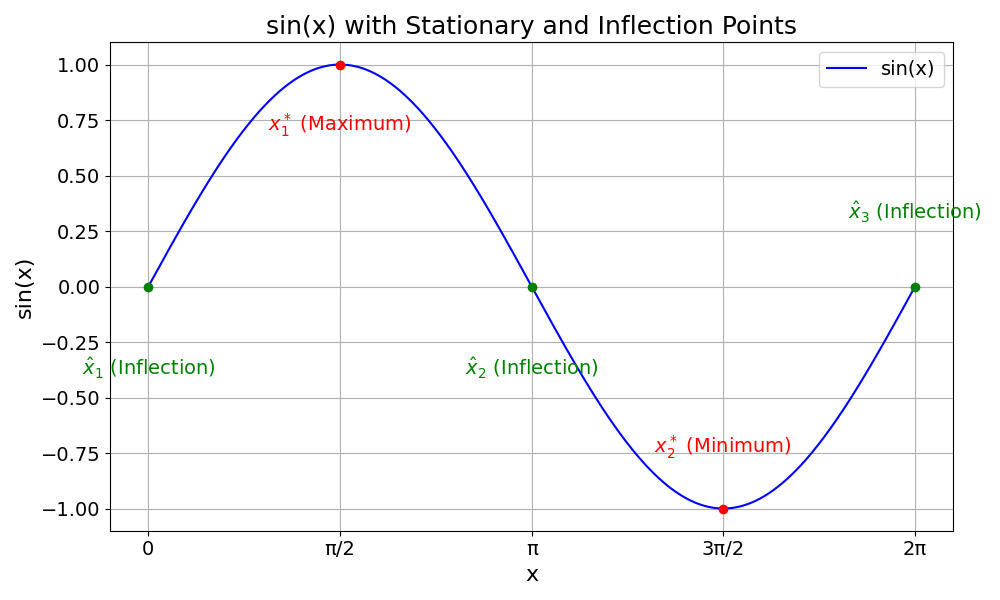
\includegraphics[width=0.5\textwidth]{generated_image.png}
    \caption{Problem 2.(d) - Graph of $\sin(x)$ with labeled stationary and inflection points.}
    \label{fig1}
    \end{figure} \\

    \noindent 3. Consider the single variable function $ f(x) = e - ax^2 $, where a is a constant. This function is often used as
    a ”radial basis function” for function approximation. Please answer the following questions completely: \\

    \noindent (a) Is the point $ x = 0 $ a stationary point for (i) $ a > 0 $, and (ii) $ a < 0 $. What happens if $ a = 0 $? Is
    $ x = 0 $ still a stationary point?

    \[
        f'(x) = -2ax \cdot e^{-ax^2}
        \]
        \[
        f'(0) = 0 \Rightarrow x = 0 \text{ is a stationary point regardless of the sign of } a.
        \]
        \[
        \text{If } a = 0, \quad f(x) = 0 \quad \text{(constant function).}
        \]
        \[
        \text{Since every point on a constant function is a stationary point, } x = 0 \text{ is still a stationary point.}
    \]

    \noindent (b) If $ x = 0 $ is a stationary point, classify it as a minimum, maximum, or an inflection point for (i)
    $ a > 0 $ ,(ii) $ a < 0 $, and (iii) $ a = 0 $.

    \[
        f''(x) = -2a e^{-ax^2} + 4a^2 x^2 e^{-ax^2} = e^{-ax^2} (-2a + 4a^2 x^2)
        \]
        \[
        = 4a^2 e^{-ax^2} \left(x^2 - \frac{1}{2a} \right)
        \]
        \[
        f''(0) = -2a
        \]
        \[
        \begin{cases}
        < 0 & \text{if } a > 0 \Rightarrow x = 0 \text{ is a local maximum} \\
        > 0 & \text{if } a < 0 \Rightarrow x = 0 \text{ is a local minimum} \\
        = 0 & \text{if } a = 0 \Rightarrow x = 0 \text{ is an inflection point}
        \end{cases}
    \]

    \noindent (c) Prepare a plot of f(x) for $ a = 1 $, $ a = 2 $, and $ a = 3 $. Plot all three curves on the same figure. By
    observing the plot, do you think $ f(x) = e - ax^2 $, $ a > 0 $ has a global minimum? If so, what is the
    value of $ x $ and $ f(x) $ at the minimum? \\
    
    Please refer to the Figure 2.
        \begin{figure}[h!]
        \centering
        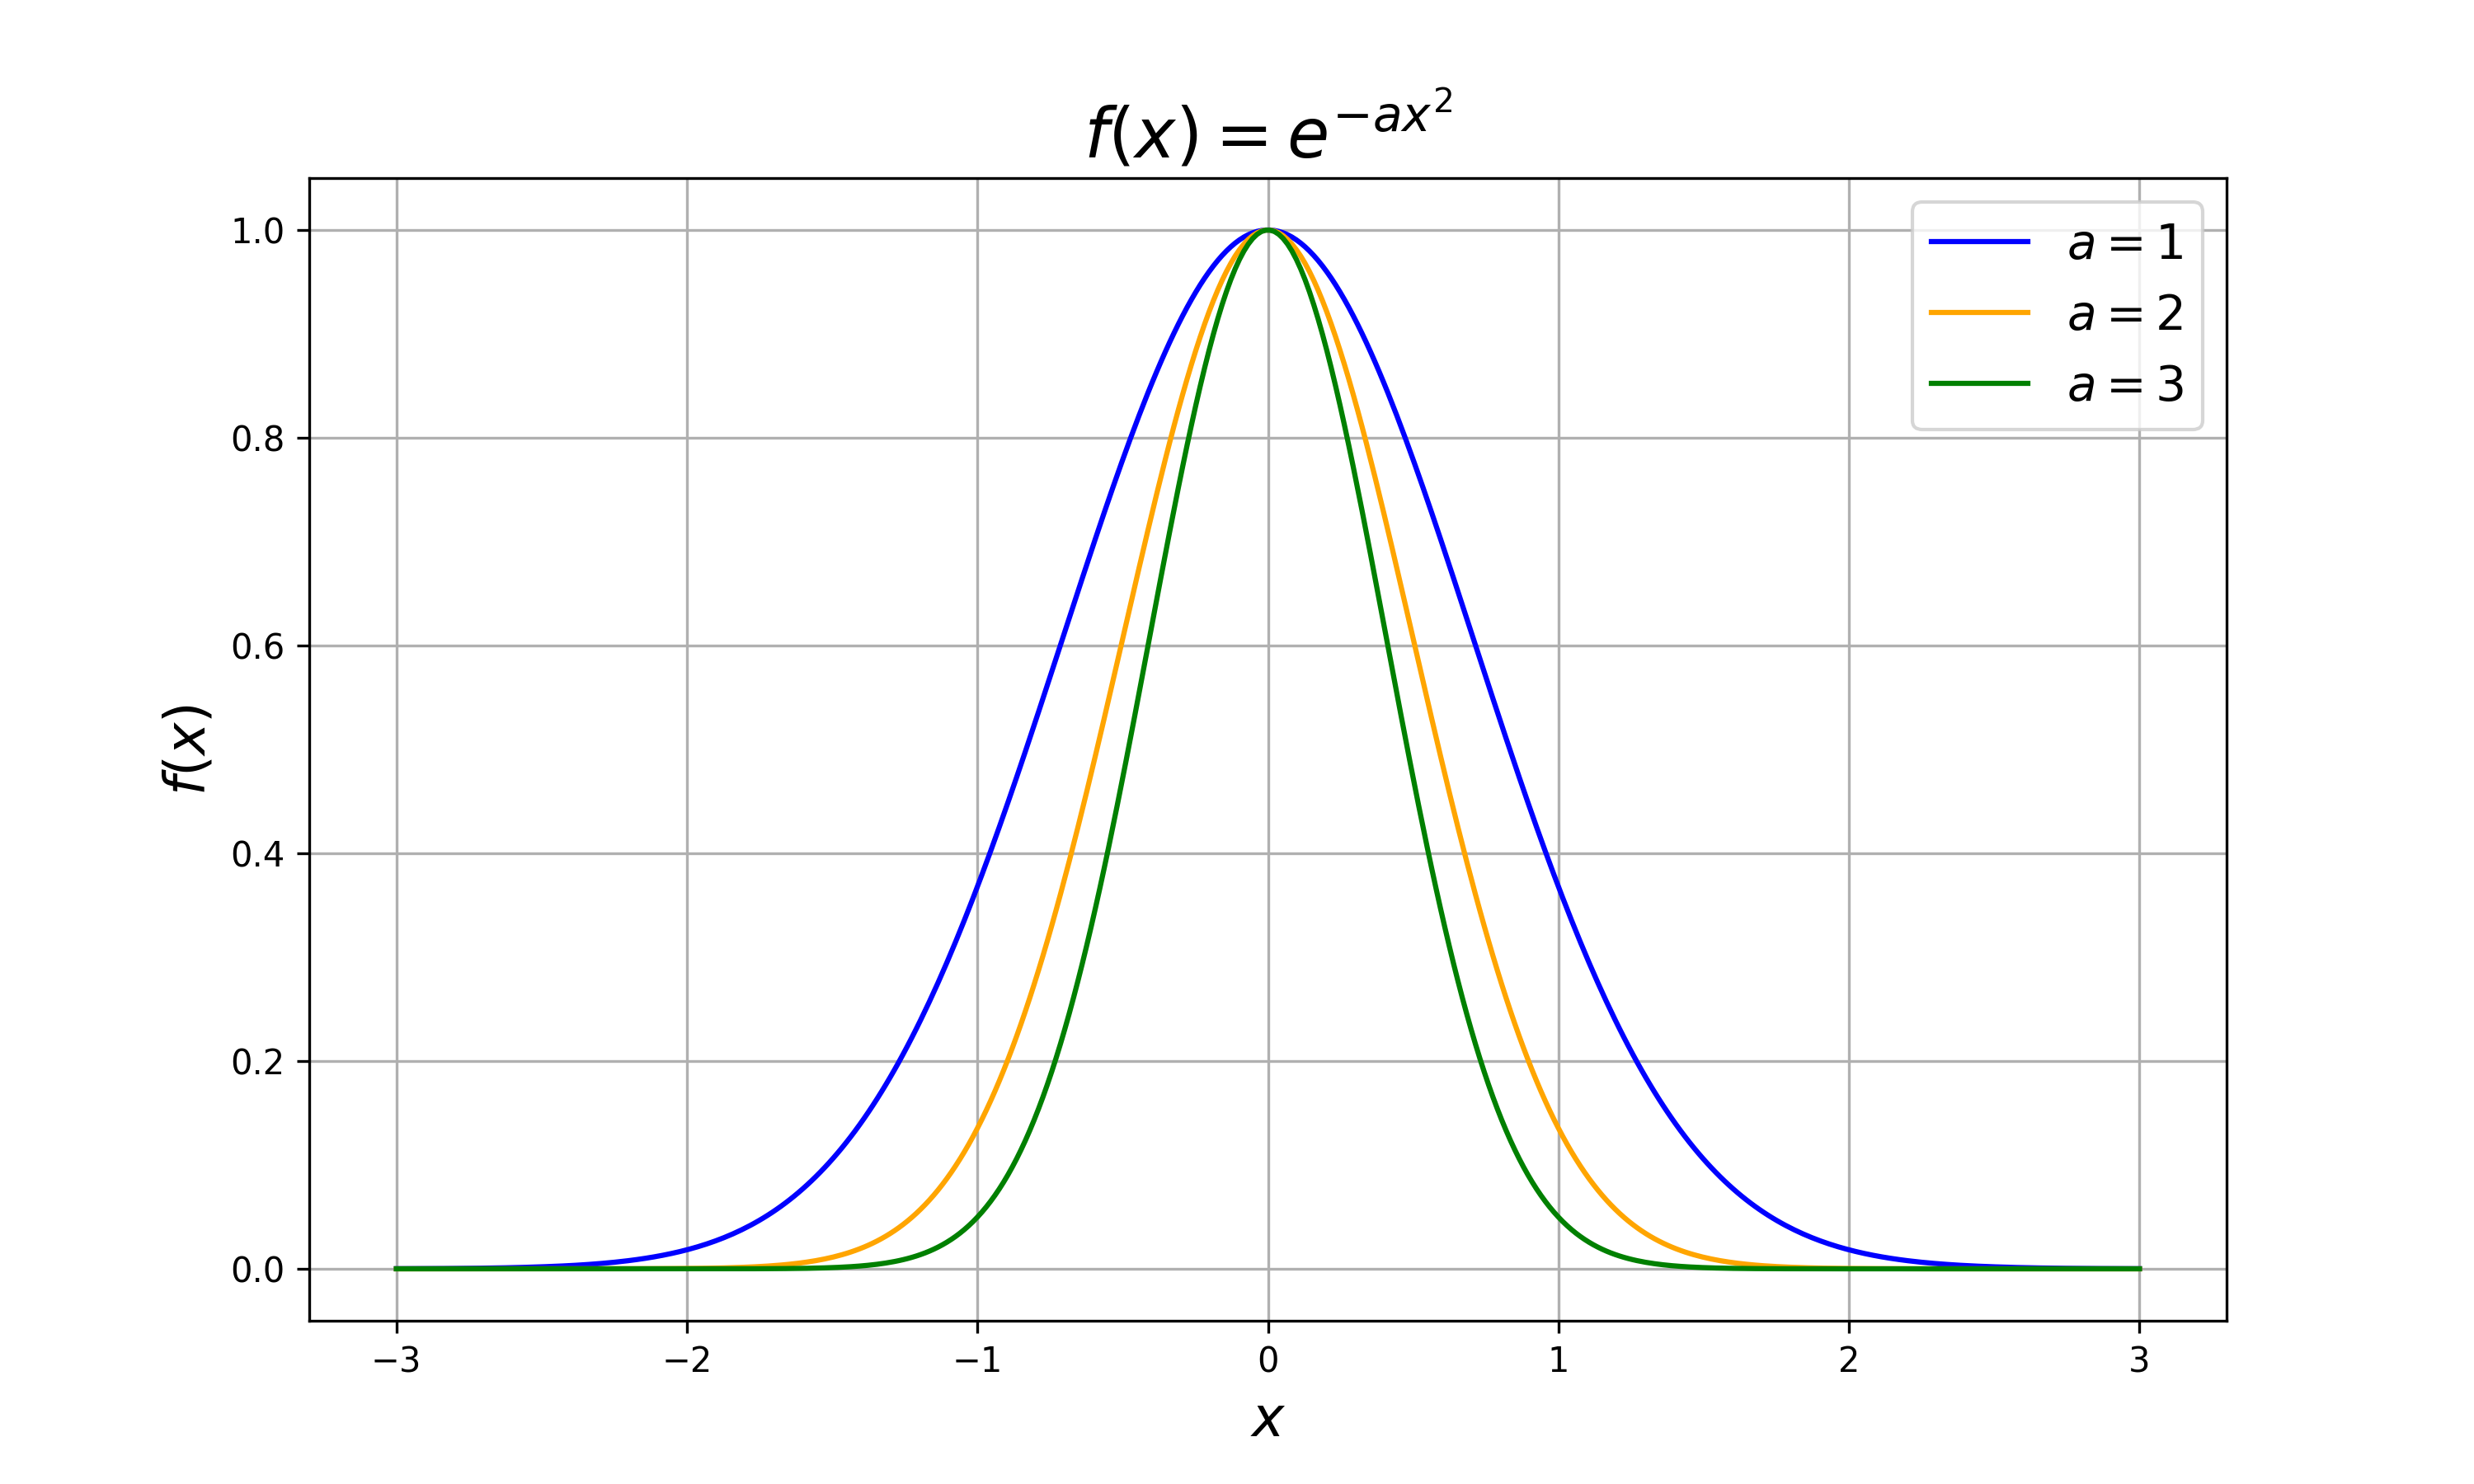
\includegraphics[width=0.5\textwidth]{generated_image2.png}
        \caption{Problem 3.(c) - Graph of $e^{-ax^2}$ with three different positive a values.}
        \label{fig2}
        \end{figure} \\
    I think $f(x)$ would have a global minimum, if certain finite boundary is given.
    If given boundary is $[-b; b]$, global minimum value will be $e^{-ab^2}$. \\

    \noindent 4. Let $ A = \begin{bmatrix} 3 & 4 \\ 2 & 1 \end{bmatrix} $ \\ % 행렬 쓰는 법
    (a) Use the definition to determine whether $ \begin{bmatrix} -\pi \\ \pi \end{bmatrix} $ and $ \begin{bmatrix} 1 \\ 2 \end{bmatrix} $
    are eigenvectors. of $ A $ associated with $ \lambda = -1 $. \\

    \[
        A \begin{bmatrix} -\pi \\ \pi \end{bmatrix}
        = \begin{bmatrix} 3 & 4 \\ 2 & 1 \end{bmatrix}
        \begin{bmatrix} -\pi \\ \pi \end{bmatrix}
        = \begin{bmatrix} -3\pi + 4\pi \\ -2\pi + \pi \end{bmatrix}
        = \begin{bmatrix} \pi \\ -\pi \end{bmatrix}
        = -1 \cdot \begin{bmatrix} -\pi \\ \pi \end{bmatrix}
    \]

    \[
        \text{Therefore, } \begin{bmatrix} -\pi \\ \pi \end{bmatrix} \text{ is an eigenvector of } A \text{ with eigenvalue } -1.
    \]

    \[
        A \begin{bmatrix} 1 \\ 2 \end{bmatrix}
        = \begin{bmatrix} 3 & 4 \\ 2 & 1 \end{bmatrix}
        \begin{bmatrix} 1 \\ 2 \end{bmatrix}
        = \begin{bmatrix} 11 \\ 4 \end{bmatrix}
        = 2 \begin{bmatrix} 1 \\ 2 \end{bmatrix}
        + \begin{bmatrix} 9 \\ 0 \end{bmatrix}
    \]

    \[
        \therefore \begin{bmatrix} 1 \\ 2 \end{bmatrix} \text{ is not an eigenvector.}
    \]

    \noindent (b) Is either of the given eigenvectors of A associated with $ \lambda = 5 $?
    \[
        \begin{bmatrix}
        3 & 4 \\
        2 & 1 
        \end{bmatrix}
        \begin{bmatrix}
        x_1 \\
        x_2 
        \end{bmatrix}
        =
        5
        \begin{bmatrix}
        x_1 \\
        x_2 
        \end{bmatrix}
    \]

    \[
        \begin{cases}
        3x_1 + 4x_2 = 5x_1 \Rightarrow x_1 = 2x_2 \\
        2x_1 + x_2 = 5x_2 \Rightarrow x_1 = 2x_2 \\
        \end{cases}
    \]

    \[
        \begin{bmatrix}
        x_1 \\
        x_2 
        \end{bmatrix}
        =
        x_2
        \begin{bmatrix}
        2 \\
        1 
        \end{bmatrix}
    \]

    \[
        \therefore \lambda = 5 \text{ is eigenvalue and } 
        \begin{bmatrix}
            2 \\
            1
        \end{bmatrix} \text{ is corresponding eigenvector.}
    \]

    \noindent (c) What is the point of this exercise?

    If either eigenvector or eigenvalue is known, the other one could be evaluated as well.\\

    \noindent 5. Use the Bisection, Fixed-Point, Newton’s, and Secant methods to find solutions accurate to within 
    $ 10^{-5} $ for the following problems: \\
    (a) $ x^2 - 4x + 4 - ln(x) = 0 $ for $ 1 \leq x \leq 2 $ and $ 2 \leq x \leq 4 $ \\
    (b) $ x + 1 - 2sin(\pi x) = 0 $ for $ 0 \leq x \leq 0.5 $ and $ 0.5 \leq x \leq 1 $ \\
    Write a code to solve the above problems using the specified methods. Provide a plot illustrating the
    convergence of the error versus the number of iterations. For the fixed-point, Newton’s, and Secant
    methods set $ x_0 $ to be the minimum point for the specified range. In addition to the plot, show a table
    with four entries of the values of $ x, f(x) $ and the error $ f(x) $. You may treat $ x $ as $ \bar{x} $ in these cases. Out
    of the four entries, provide the initial value, the final values and two intermediary values during the
    convergence of the algorithm. \\

    Please refer to the Figure 3 to see the plot of convergence error versus iterations of each method, 
    and refert to the Table 1, 2, 3, 4 to see the comparison between Fixed-point iteration method and Newton's method.
    Please refer to the Appendix section to see the code(Python-based) corresponding to each method.

    \clearpage
    \begin{figure}[h!]
    \centering
    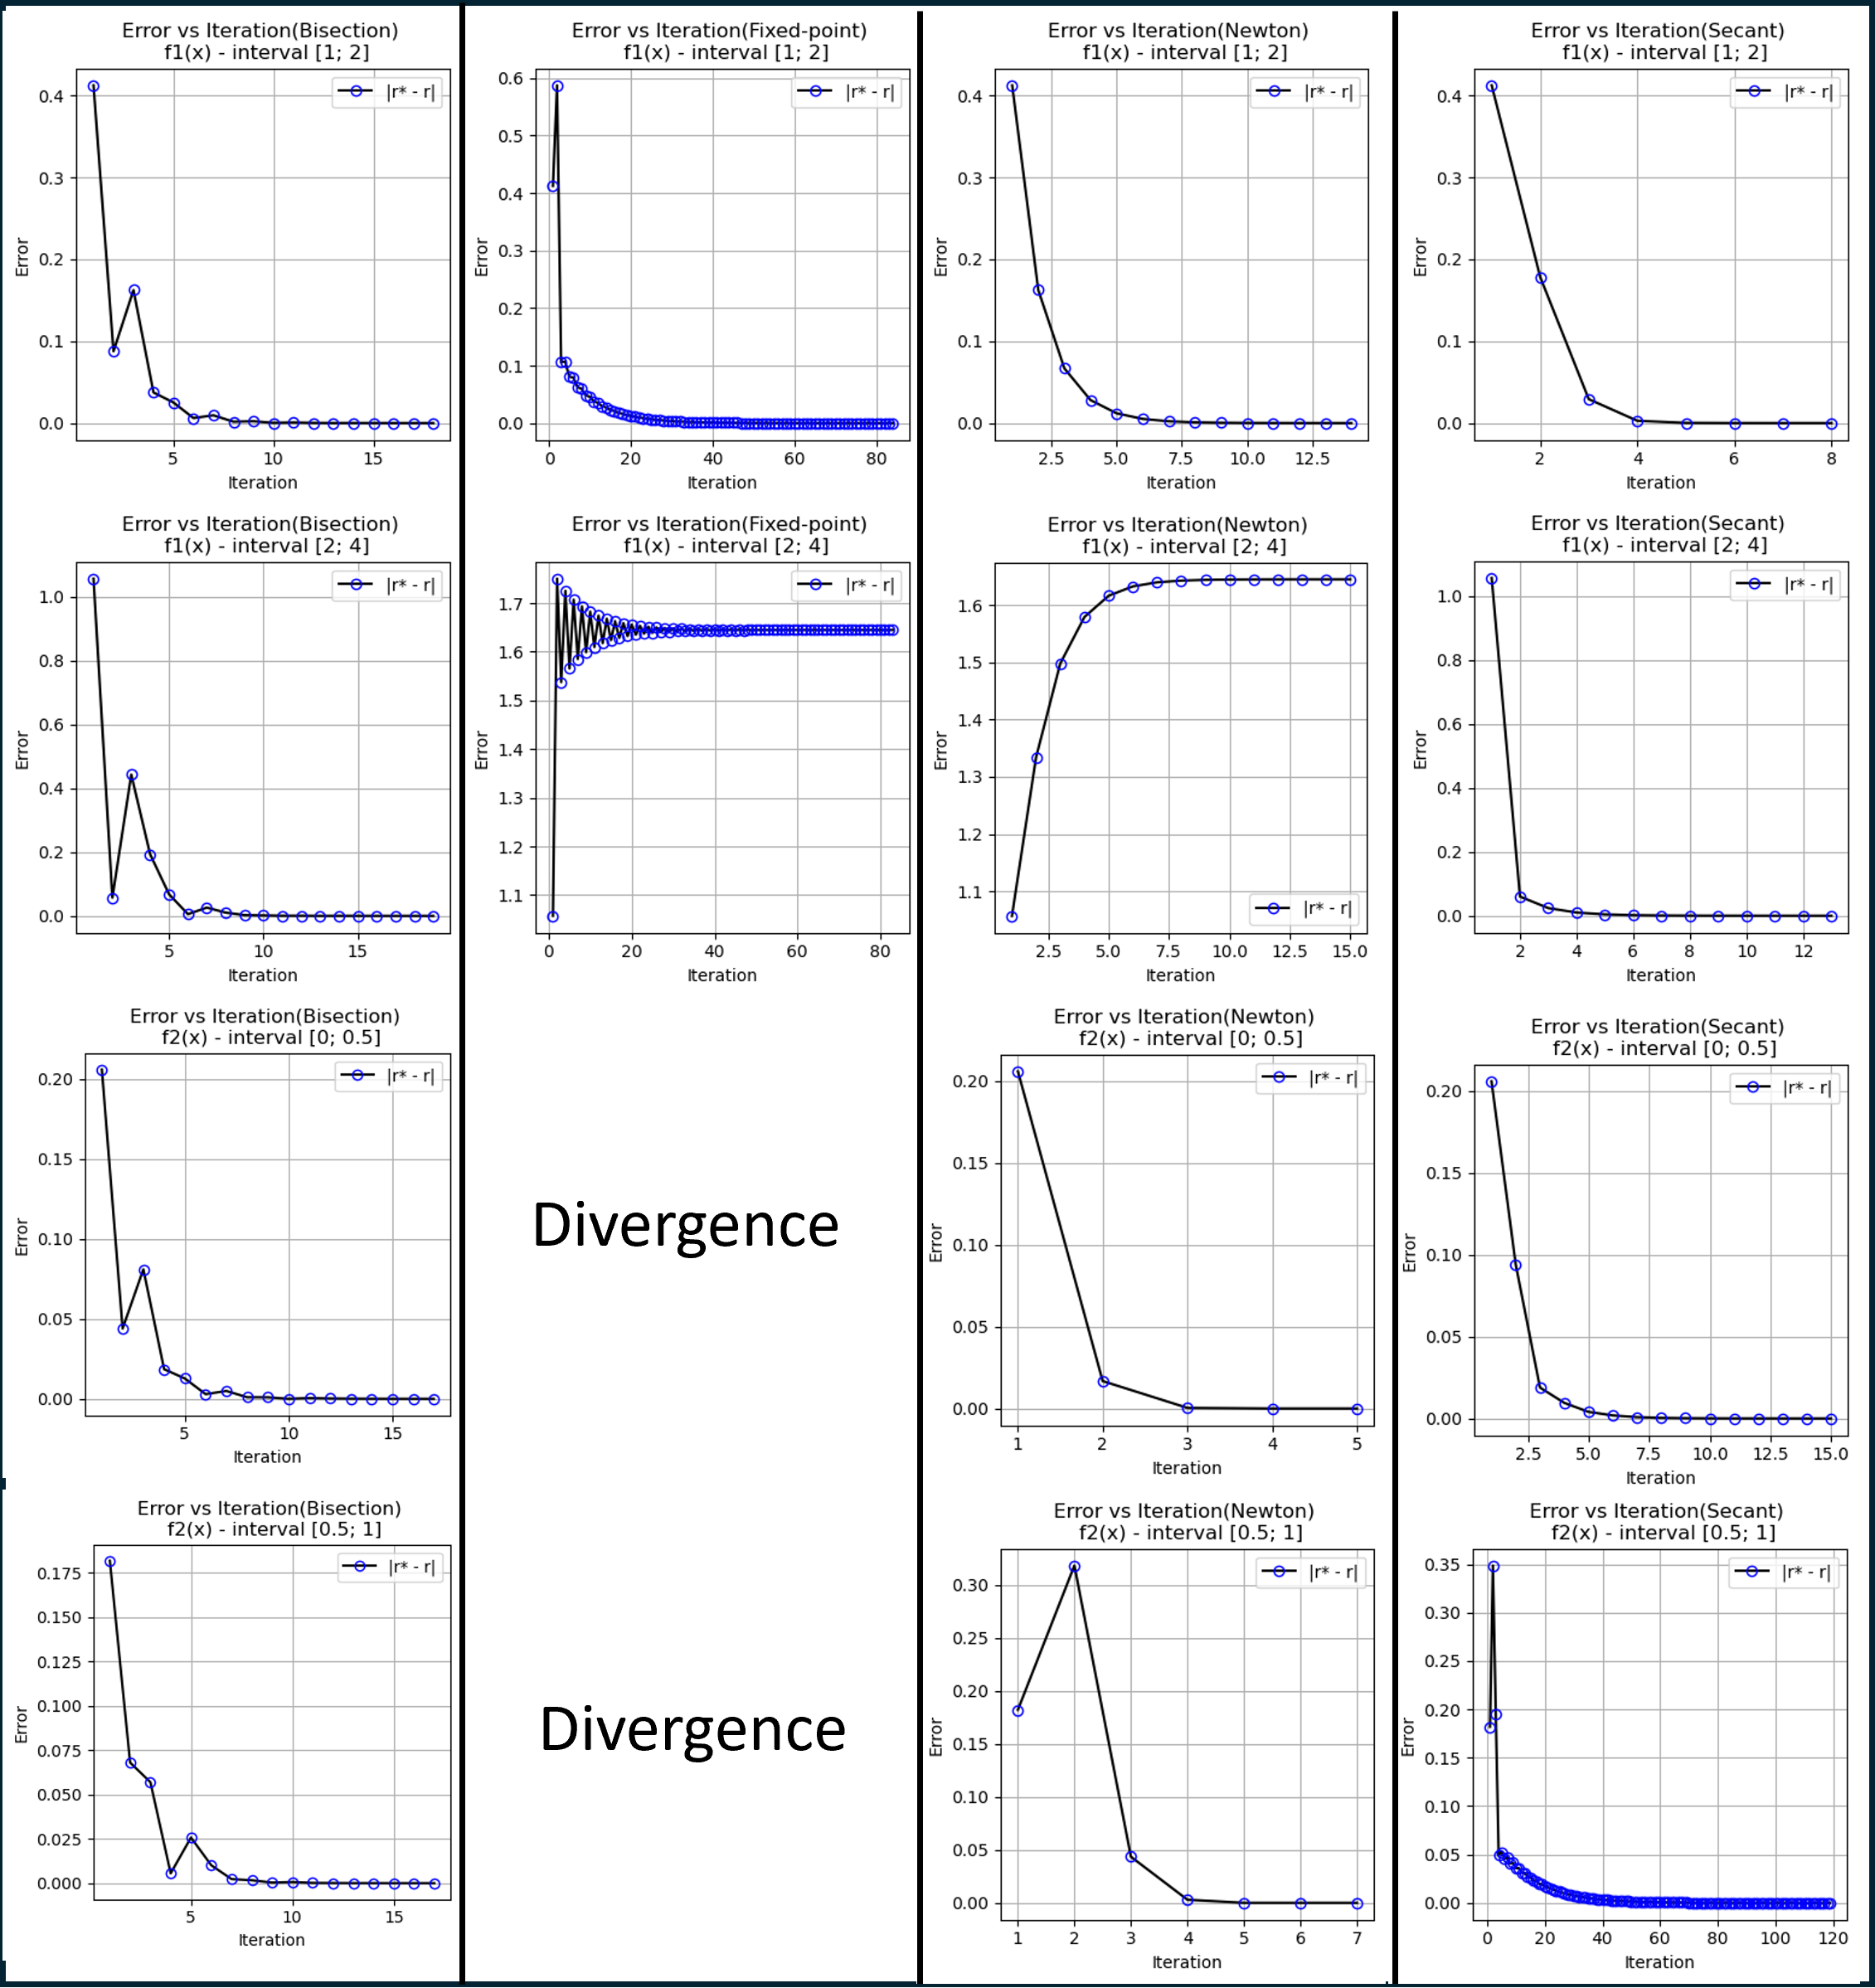
\includegraphics[width=1\textwidth]{generated_image4.png}
    \caption{Problem 5 - Error vs Iteration plot of Bisection, Fixed-point iteration, Newton's, Secant method.}
    \label{fig3}
    \end{figure}

    \clearpage
    \begin{table}[h!]
        \centering
        \begin{tabular}{cccc}
        \toprule
        Iteration ($k$) & $r$ & $f(r)$ & $|r^* - r|$ \\
        \midrule
        0 & 2.000000 & 0.693147 & 1.057104 \\
        1 & 1.306853 & 0.212831 & 1.750251 \\
        2 & 1.519684 & 0.187799 & 1.537420 \\
        Final & 1.412396 & $8.36 \times 10^{-6}$ & 1.644708 \\
        \bottomrule
        \end{tabular}
        \caption{Problem 5 - Fixed-Point Iteration for $f_1(x)$ on $[2, 4]$}
        \label{tab:fixed_f1}
        \end{table}

        \begin{table}[h!]
        \centering
        \begin{tabular}{cccc}
        \toprule
        Iteration ($k$) & $r$ & $f(r)$ & $|r^* - r|$ \\
        \midrule
        0 & 2.000000 & 0.693147 & 1.057104 \\
        1 & 1.722741 & 0.467044 & 1.334362 \\
        2 & 1.559309 & 0.250035 & 1.497794 \\
        Final & 1.412397 & $1.15 \times 10^{-5}$ & 1.644706 \\
        \bottomrule
        \end{tabular}
        \caption{Problem 5 - Newton's Method for $f_1(x)$ on $[2, 4]$}
        \label{tab:newton_f1}
        \end{table}

        \begin{table}[h!]
        \centering
        \begin{tabular}{cccc}
        \toprule
        Iteration ($k$) & $r$ & $f(r)$ & $|r^* - r|$ \\
        \midrule
        0 & 0.000000 & 1.000000 & 0.206035 \\
        1 & 1.000000 & 2.000000 & 0.793965 \\
        2 & 3.000000 & 4.000000 & 2.793965 \\
        Final & \text{Diverge} & \text{Diverge} & \text{Diverge} \\
        \bottomrule
        \end{tabular}
        \caption{Problem 5 - Fixed-Point Iteration for $f_2(x)$ on $[0, 0.5]$}
        \label{tab:fixed_f2}
        \end{table}

        \begin{table}[h!]
        \centering
        \begin{tabular}{cccc}
        \toprule
        Iteration ($k$) & $r$ & $f(r)$ & $|r^* - r|$ \\
        \midrule
        0 & 0.000000 & 1.000000 & 0.206035 \\
        1 & 0.189280 & 0.068859 & 0.016755 \\
        2 & 0.205656 & 0.001520 & 0.000379 \\
        Final & 0.206035 & $2.68 \times 10^{-13}$ & $3.84 \times 10^{-13}$ \\
        \bottomrule
        \end{tabular}
        \caption{Problem 5 - Newton's Method for $f_2(x)$ on $[0, 0.5]$}
        \label{tab:newton_f2}
    \end{table}

    \noindent 6. Let $ f(x, y) = x^3 - x + y^3 - y $

    \noindent(a) Graph the surface $ z = f(x, y) $. \\

    Please refer to the Figure 4. \\

    \begin{figure}[h!]
    \centering
    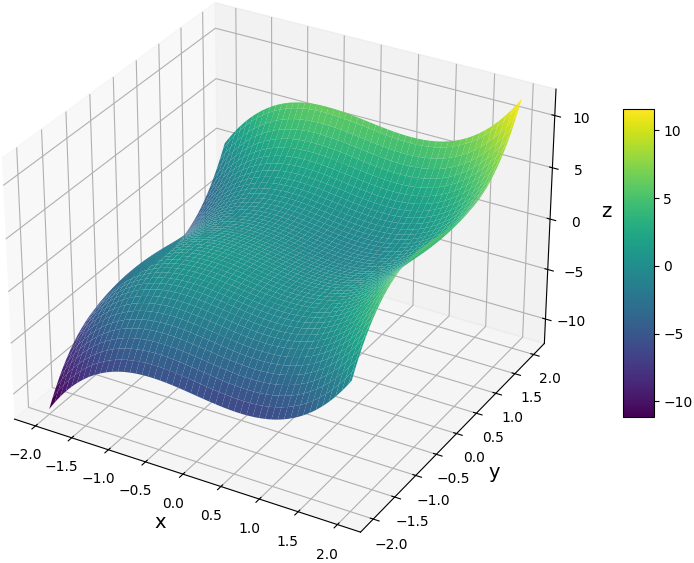
\includegraphics[width=0.7\textwidth]{generated_image3.png}
    \caption{Problem 6.(a) - Graph of $f(x, y) = x^3 - x + y^3 - y$}
    \label{fig4}
    \end{figure}

    \noindent (b) Verify that the complete list of critical points of $ f $ is
    \( % 문장 안에 수식 넣는 법 ; inline 수식 방식
    \left(-\frac{1}{\sqrt{3}}, -\frac{1}{\sqrt{3}}\right),\ % 수식에 맞춰서 괄호 크기 자동 조정 ; 분수 표기
    \left(-\frac{1}{\sqrt{3}}, \frac{1}{\sqrt{3}}\right),\ 
    \left(\frac{1}{\sqrt{3}}, -\frac{1}{\sqrt{3}}\right),\ 
    \left(\frac{1}{\sqrt{3}}, \frac{1}{\sqrt{3}}\right)
    \)

    \[ \text{First derivatives: }
    \frac{\partial f}{\partial x} = 3x^2 - 1=0, 
    \frac{\partial f}{\partial y} = 3y^2 - 1=0 \]
    \[ \text{Critical points: }
    \left( \pm \frac{1}{\sqrt{3}}, \pm \frac{1}{\sqrt{3}} \right) \]

    \noindent (c) Calculate the Hessian matrix

    \[ \text{Hessian: }
    H = \begin{bmatrix}
    6x & 0 \\
    0 & 6y
    \end{bmatrix} \]
    \[ \text{At } \left( \frac{1}{\sqrt{3}}, \frac{1}{\sqrt{3}} \right):
    H = \begin{bmatrix} 2\sqrt{3} & 0 \\ 0 & 2\sqrt{3} \end{bmatrix}, \lambda_1,\lambda_2 > 0 \Rightarrow \text{Local Min} \]
    \[ \text{At } \left( -\frac{1}{\sqrt{3}}, -\frac{1}{\sqrt{3}} \right):
    H = \begin{bmatrix} -2\sqrt{3} & 0 \\ 0 & -2\sqrt{3} \end{bmatrix}, \lambda_1,\lambda_2 < 0 \Rightarrow \text{Local Max} \]
    \[ \text{At } \left( \pm \frac{1}{\sqrt{3}}, \mp \frac{1}{\sqrt{3}} \right): 
    H = \begin{bmatrix} \pm 2\sqrt{3} & 0 \\ 0 & \mp 2\sqrt{3} \end{bmatrix}, \text{Eigenvalues of opposite sign} \Rightarrow \text{Saddle Point} \]

    \noindent (d) Fill in the following table. \\

    \begin{tabular}{|c|c|c|c|}
        \hline
        Critical points & Hessian at $ (x, y) $ & Eigenvalues of Hessian at $ (x, y) $ & Concavity at $ (x, y) $ \\
        \hline
        $ \left(-\frac{1}{\sqrt{3}}, -\frac{1}{\sqrt{3}}\right) $ & $\begin{bmatrix} -2\sqrt{3} & 0 \\ 0 & -2\sqrt{3} \end{bmatrix}$ & $-2\sqrt{3}, -2\sqrt{3}$ & Concavity \\
        \hline
        $ \left(-\frac{1}{\sqrt{3}}, \frac{1}{\sqrt{3}}\right) $ & $\begin{bmatrix} -2\sqrt{3} & 0 \\ 0 & 2\sqrt{3} \end{bmatrix}$ & $-2\sqrt{3}, 2\sqrt{3}$ & Saddle \\
        \hline
        $ \left(\frac{1}{\sqrt{3}}, -\frac{1}{\sqrt{3}}\right) $ & $\begin{bmatrix} 2\sqrt{3} & 0 \\ 0 & -2\sqrt{3} \end{bmatrix}$ & $2\sqrt{3}, -2\sqrt{3}$ & Saddle \\
        \hline
        $ \left(\frac{1}{\sqrt{3}}, \frac{1}{\sqrt{3}}\right) $ & $\begin{bmatrix} 2\sqrt{3} & 0 \\ 0 & 2\sqrt{3} \end{bmatrix}$ & $2\sqrt{3}, 2\sqrt{3}$ & Convexity \\
        \hline
    \end{tabular} \\

    \noindent (e) Examine the table carefully and explain how eigenvalues of Hessian matrices can help you classify
    the concavity of the surface at each critical point.\\

    If eigenvalues are all positive, the function has local minimum and convexity at that point. \\
    If eigenvalues are all negative, the function has local maximum and concavity at that point. \\
    If eigenvalues are mixed with positive and negative, the function has saddle point. \\

    \noindent 7. Find the critical points of $ f(x, y) = x^2 + y^3 - x^2y + xy^2 $ and classify them all by using the eigenvalues
    of the appropriate Hessian matrices. \\

    The partial derivatives are:
    \[ \frac{\partial f}{\partial x} = - 2 x y + 2 x + y^{2} \]
    \[ \frac{\partial f}{\partial y} = - x^{2} + 2 x y + 3 y^{2} \]

    We solve the coupled equation:
    \[ \frac{\partial f}{\partial x} = 0, \quad \frac{\partial f}{\partial y} = 0 \]

    \[ \frac{\partial f}{\partial x} = 2x - 2xy + y^2 = 0 \\\\
    \rightarrow 2x(1 - y) + y^2 = 0 \\\\
    \rightarrow x = \frac{y^2}{2(y - 1)} \]
    \[ \frac{\partial f}{\partial y} = 3y^2 - x^2 + 22xy = 0 \\\\
    \rightarrow 3y^2 - \frac{y^4}{4(y - 1)^2} + \frac{2y^3}{2(y - 1)} = 0 \\\\[10pt]
    \rightarrow y^2 \left(3 - \frac{y^2}{4(y - 1)^2} + \frac{y}{y - 1} \right) = 0 \\\\\]
    \[ \rightarrow y^2 \left(12(y - 1)^2 - y^2 + 4y(y - 1) \right) = 0 \\\\[10pt]
    \rightarrow y^2 (15y^2 - 28y + 12) = 0 \\\\[10pt]
    \rightarrow y^2{(3y - 2)(5y - 6)} = 0 \\\]
    \[ \rightarrow y_1 = 0, \quad y_2 = \frac{2}{3}, \quad y_3 = \frac{6}{5} \]

    \begin{itemize}
    \item Critical point: $(x, y) = (- \frac{2}{3}, \frac{2}{3})$
    \item Critical point: $(x, y) = (0, 0)$
    \item Critical point: $(x, y) = (\frac{18}{5}, \frac{6}{5})$
    \end{itemize}

    Hessian matrix at $(x, y)$ : \[ H(x, y) = \begin{bmatrix}
        2 - 2y & -2x + 2y \\
        -2x + 2y & 2x + 6y
    \end{bmatrix} \]

    At the critical point $(x, y) = (- \frac{2}{3}, \frac{2}{3})$:

    Hessian :
    \[
    H = \left[\begin{matrix}\frac{2}{3} & \frac{8}{3}\\\frac{8}{3} & \frac{8}{3}\end{matrix}\right]
    \]

    Eigenvalues:
    \[
    \frac{5}{3} - \frac{\sqrt{73}}{3}, \frac{5}{3} + \frac{\sqrt{73}}{3}
    \]
    Classification: 	Saddle point\
    \bigskip

    At the critical point $(x, y) = (0, 0)$:

    Hessian matrix:
    \[
    H = \left[\begin{matrix}2 & 0\\0 & 0\end{matrix}\right]
    \]

    Eigenvalues:
    \[
    2, 0
    \]
    Classification: 	Indeterminate\
    \bigskip

    At the critical point $(x, y) = (\frac{18}{5}, \frac{6}{5})$:

    Hessian matrix:
    \[
    H = \left[\begin{matrix}- \frac{2}{5} & - \frac{24}{5}\\- \frac{24}{5} & \frac{72}{5}\end{matrix}\right]
    \]

    Eigenvalues:
    \[
    7 - \frac{\sqrt{1945}}{5}, 7 + \frac{\sqrt{1945}}{5}
    \]
    Classification: 	Saddle point\
    \bigskip

}   

\clearpage
\section*{Appendix}
\addcontentsline{toc}{section}{Appendix}
Here is the Python code regarding the problem 5.

\begin{verbatim}
def bisection(func, a0, b0, tol):
    if func(a0)*func(b0) < 0:
        list_k, list_r, list_f = [0], [a0], [func(a0)]
        a_new = a0
        b_new = b0
        k = 0
        err = np.abs(b_new - a_new)
        while err > tol:
            k = k + 1; list_k.append(k)
            a_old = a_new
            b_old = b_new
            mid = .5*(a_old + b_old); list_r.append(mid)
            f_a_old = func(a_old)
            f_b_old = func(b_old)
            f_mid = func(mid); list_f.append(np.abs(f_mid))
            if f_mid == 0:
                err = 0
                print(f"At {k:d}-th iteration : The root of which function value is exactly zero is acquired so iteration ends ! ")
                break
            sign_w_a = f_mid*f_a_old
            sign_w_b = f_mid*f_b_old
            if (sign_w_a < 0) & (sign_w_b > 0):
                b_new = mid
                a_new = a_old
            elif (sign_w_a > 0) & (sign_w_b < 0):
                a_new = mid
                b_new = b_old
            err = abs(a_new - b_new)
            print(f"At {k:d}-th iteration : a_new, b_new of interval are {a_new:.6f}, {b_new:.6f} and the interval length is {err:.6f}")
        if f_mid == 0:
            r = mid
            print(f"Converged to Exact Root. {k:d}-th iteration / r = {r:.6f} / func(r) = {func(r):.6f}")
        else:
            r = .5*(a_new + b_new)
            print(f"Converged by Tolerance. {k:d}-th iteration / r = {r:.6f} / func(r) = {func(r):.6f} / length_interval = {err:.6f}")
        return r, np.array(list_k), np.array(list_r), np.array(list_f)
    else:
        print(f"f(a0)*f(b0) is positive. There may not be root in [{a0}; {b0}]. Try another bracket !")
--------------------------------------------------------------------------------------------------------------------------
def fixed_point(func, r0, tol):
g = lambda x : func(x) + x
r_new = r0
k = 0
err = 1
list_k, list_r, list_f = [k], [r0], [func(r0)]
while err > tol:
    k = k + 1; list_k.append(k)
    r_old = r_new
    r_new = g(r_old); list_r.append(r_new); list_f.append(func(r_new))
    err = np.abs(r_new - r_old)
    if err < tol:
        print(f"Converged By Tolerance. {k:d}-th iteration / r = {r_new:.6f} / f(r) = {f(r_new):.6f} / |r_new - r_old| = {err:.6f}")
        return r_new, np.array(list_k), np.array(list_r), np.array(list_f)
    else:
        print(f"At {k:d}-th iteration : r_new is {r_new:.6f} and the |r_new - r_old| is {err:.6f}")
--------------------------------------------------------------------------------------------------------------------------
def newton(func, Dfunc, r0, tol):
r_new = r0
k = 0
err = 1
list_k, list_r, list_f = [k], [r0], [func(r0)]
while err > tol:
    k = k + 1; list_k.append(k)
    r_old = r_new
    r_new = r_old - func(r_old)/Dfunc(r_old); list_r.append(r_new); list_f.append(func(r_new))
    err = np.abs(r_new - r_old)
    if err < tol:
        print(f"Converged By Tolerance. {k:d}-th iteration / r = {r_new:.6f} / f(r) = {func(r_new):.6f} / |r_new - r_old| = {err:.6f}")
        return r_new, np.array(list_k), np.array(list_r), np.array(list_f)
    else:
        print(f"At {k:d}-th iteration : r_new is {r_new:.6f} and the |r_new - r_old| is {err:.6f}")
--------------------------------------------------------------------------------------------------------------------------
def secant(func, r0, r1, tol):
r_old = r0
r_new = r1
k = 0
err = np.abs(r_new - r_old)
list_k, list_r, list_f = [k], [r0], [func(r0)]
while err > tol:
    k = k + 1; list_k.append(k)
    r_older = r_old
    r_old = r_new
    r_new = r_old - func(r_old)/(func(r_old) - func(r_older)/(r_old - r_older)); list_r.append(r_new); list_f.append(func(r_new))
    err = np.abs(r_new - r_old)
    if err < tol:
        print(f"Converged By Tolerance. {k:d}-th iteration / r = {r_new:.6f} / f(r) = {func(r_new):.6f} / |r_new - r_old| = {err:.6f}")
        return r_new, np.array(list_k), np.array(list_r), np.array(list_f)
    else:
        print(f"At {k:d}-th iteration : r_new is {r_new:.6f} and the |r_new - r_old| is {err:.6f}")
\end{verbatim}

\end{document}